\documentclass{article}
\usepackage[utf8]{inputenc}
\usepackage{graphicx} 
\usepackage{fancyhdr}
\usepackage{ragged2e}
\usepackage{multirow}
\usepackage[hidelinks]{hyperref}
\usepackage[table,xcdraw]{xcolor}
\usepackage{ulem}
\usepackage{listings}
\usepackage[spanish]{babel} % Paquete para idioma español
\usepackage{xcolor} % Para usar colores

\usepackage{pgfgantt}
\usepackage{float}
\usepackage{pdflscape} % Paquete para la orientación horizontal
\usepackage{longtable} % Para tablas largas.
\usepackage{geometry} 
\usepackage{ragged2e}
\usepackage{translator}
\ganttset{calendar week text={\small{\startday/\startmonth}}}
\newcommand\textganttbar[5][]{%
    \ganttbar[#1,bar/.append style={alias=tmp}]{#2}{#4}{#5}
    \path 
    let
    \p1=(tmp.west),\p2=(tmp.east),
    \n1={\x2-\x1},\n2={width("#3")},
    \n3={ifthenelse(\n1>\n2,90,270)}
    in
    node [anchor=\n3,font=\footnotesize] at (tmp.north) {#3};
}


%               Comandos Personalizados



% Adicionales
\addto\captionsspanish{\renewcommand{\contentsname}{Índice}} % Cambio de  Adicionales Contents a Indice
\pagestyle{fancy}
\fancyhf{}
\lhead{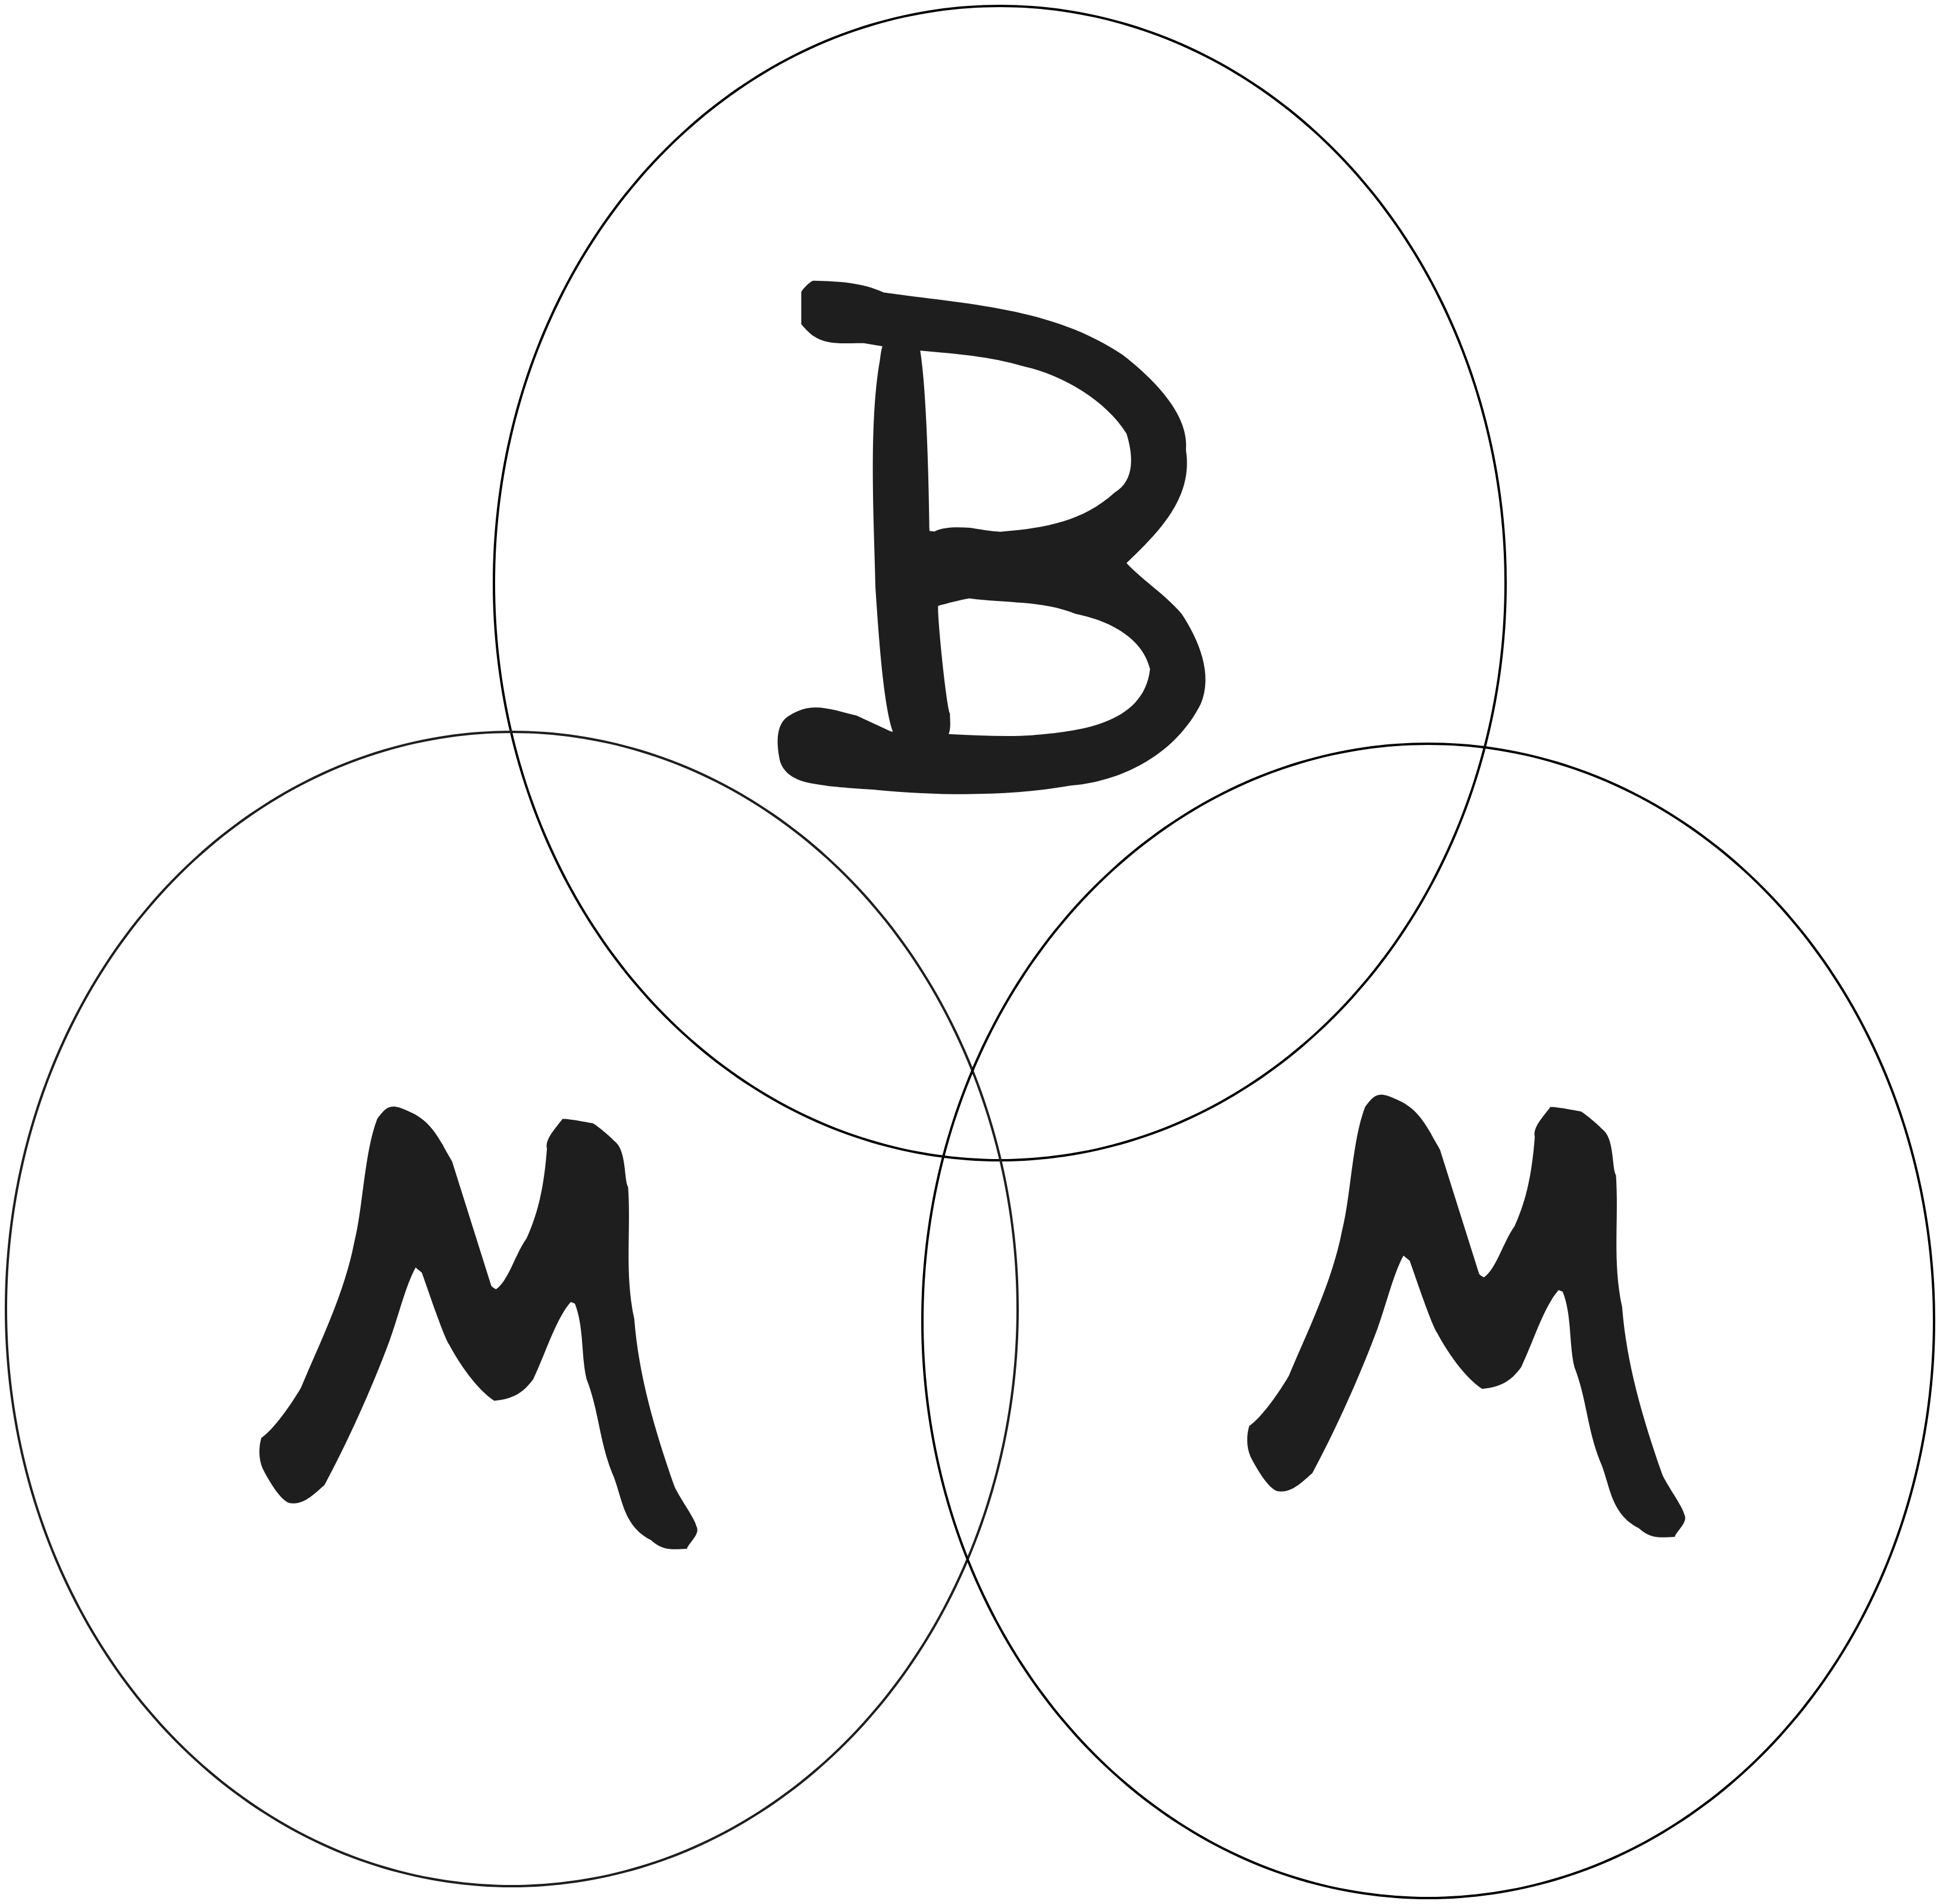
\includegraphics[width=1cm]{TFG/Logo.png}}

\renewcommand{\headrulewidth}{3pt}
   %Comienzo de Documento
    \begin{document}
            % Creacion de Portada----------------------------------------------------------
% Comienzo de Documento
    % Creación de Portada
    \begin{titlepage}
        \begin{center}
            {\scshape\large{Grado Superior}}\\
            {\scshape\large{Desarrollo de aplicaciones multiplataforma}} \\

            
            \vspace{2cm}
            {
\includegraphics[width=0.4\textwidth]{TFG/fotomain.png}} \par
            \vspace{2cm}
            {\scshape\large{ Aplicación para la Gestión de Tareas y Control \\ de Alimentos en el Hogar}\\
            \vspace{2cm}
            \textbf{TaskTracer}}} \\
            \vspace{2cm}
            {\Large Autor:} \\
            \vspace{1mm}
            {\Large Borja Merchán Mckenna} \\
            \vspace{1mm}
            {\Large 27/10/2024}
        \end{center}
    \end{titlepage}

 % ----------------------------------------------------------------
        %Comienzo de Toc
        
        \clearpage
        \tableofcontents

         \clearpage

\section{Descripción del Proyecto}
Tasktracer es una aplicación multiplataforma diseñada para gestionar tareas diarias y controlar el inventario de alimentos en el hogar. La funcionalidad principal incluye:
\begin{itemize}

    \item \textbf{Creación de Usuarios:} Los usuarios podrán registrarse y autenticarse utilizando Firebase.
    \item \textbf{Grupos de Hogar:} Los usuarios podrán crear grupos o unirse de hogar para gestionar de manera colaborativa tanto el "to-do" del hogar como el inventario, permitiendo así una mejor organización.
    
    \item \textbf{Gestión de Tareas:} Permite a los usuarios crear, editar y eliminar tareas en un sistema de "to-do".
    \item \textbf{Control de Inventario:} Ofrece una visualización de productos en la nevera a través de un enfoque visual tipo Kanban, facilitando así la planificación de compras y evitando desperdicios.

\end{itemize}

   

      
\section{Tecnologías a Utilizar}
\begin{itemize}
    \item \textbf{Framework:} Flutter
    \item \textbf{Lenguaje de Programación:} Dart
    \item \textbf{Base de Datos:} Firebase (incluyendo Firebase Authentication y Firestore)
    \item \textbf{Entorno de Desarrollo:} Visual Studio Code
    \item \textbf{Documentación:} LaTeX
    \item \textbf{Control de Versiones:} GitLab
    \item \textbf{Diseño de Interfaz:} Figma
    \clearpage
    \item \textbf{Diagrama de Grant:} ideado desde el comienzo con tareas esenciales y una fecha límite aproximada, para poder controlar todo el proceso de tareas y tiempos de trabajo


  \begin{figure}[H]
            \begin{ganttchart}[
            x unit=0.120cm, % distancia entre cada unidad horizontal (días).
            y unit chart=0.4cm, % altura de cada unidad vertical.
            y unit title=0.7cm, % altura de las filas de títulos.
            title height=1, % separación entre una fila de títulos y otra (1 = ninguna separación).
            hgrid, % dibujar las separaciones verticales.
            vgrid={*6{draw=none}, dotted}, % dibujar las separaciones verticales en intervalos semanales.
            bar/.append style={fill=white}, % barras de color blanco por defecto.
            group peaks width=3,
            group peaks tip position=0.5,
            group peaks height=.1, % distintos parámetros para el formato de los grupos.
            time slot format=isodate, % formato de las fechas.
            ] {2024-09-26}{2024-12-15} % inicio y final del eje temporal (año-mes-día).

            % Títulos:
            \gantttitle{Diagrama de Gantt: TaskTracer}{81} \\ % Título centrado y extendido
            \gantttitlecalendar{year, month=shortname} \\ 
            \gantttitlecalendar[title height=2, title label node/.append style={rotate=90}]{week} \\
            \gantttitle[title/.style={opacity=0}]{}{364} \\ 

            % Grupos y tareas:
            \ganttgroup{Inicio de la Aplicación}{2024-09-26}{2024-09-29} \\
            \ganttbar[bar/.append style={fill=blue!20}]{Nombre de la aplicación}{2024-09-26}{2024-09-26} \\
            \ganttbar[bar/.append style={fill=blue!20}]{Logo de la aplicación}{2024-09-27}{2024-09-28} \\
            \ganttbar[bar/.append style={fill=blue!20}]{Investigación de herramientas}{2024-09-28}{2024-09-29} \\

            \ganttgroup{Diseño de Aplicación}{2024-09-30}{2024-10-16} \\
            \ganttbar[bar/.append style={fill=orange!50}]{Diagrama de Gantt}{2024-09-30}{2024-10-04} \\
            \ganttbar[bar/.append style={fill=orange!50}]{Diagrama de flujo}{2024-10-05}{2024-10-08} \\
            \ganttbar[bar/.append style={fill=orange!50}]{Diseñar en Figma}{2024-10-09}{2024-10-12} \\
            \ganttbar[bar/.append style={fill=orange!50}]{Diseñar en el front}{2024-10-12}{2024-10-16} \\

            \ganttgroup{Desarrollo}{2024-10-17}{2024-11-20} \\
            \ganttbar[bar/.append style={fill=green!50}]{Desarrollo de usuarios}{2024-10-17}{2024-10-22} \\
            \ganttbar[bar/.append style={fill=green!50}]{Desarrollo de grupo de hogar}{2024-10-23}{2024-10-28} \\
            \ganttbar[bar/.append style={fill=green!50}]{Desarrollo del to-do}{2024-10-29}{2024-11-03} \\
            \ganttbar[bar/.append style={fill=green!50}]{Desarrollo gestión de nevera}{2024-11-04}{2024-11-09} \\
            \ganttbar[bar/.append style={fill=green!50}]{Desarrollo de ajustes}{2024-11-10}{2024-11-20} \\ 


             \ganttgroup{Prubas}{2024-11-20}{2024-12-10} \\
            \ganttbar[bar/.append style={fill=red!50}]{Comprobación del Codigo}{2024-11-20}{2024-12-10} \\ 

            \ganttbar[bar/.append style={fill=green!50}]{Documentación en PDF}{2024-11-20}{2024-12-15} \\ 
            \ganttbar[bar/.append style={fill=green!50}]{Presentación en PowerPoint}{2024-12-10}{2024-12-15} \\ 


            % Relaciones de dependencia:

            \end{ganttchart}
            \caption{Diagrama de Gantt de TaskTracer}
            \label{fig:gantt}
        \end{figure}

\end{itemize}

\section{Justificación de los Módulos Profesionales}


La elección de estas tecnologías está alineada con los módulos del ciclo de Desarrollo de Aplicaciones Multiplataforma, ya que se busca:
\begin{itemize}
    \item Implementar aplicaciones usando frameworks modernos (Flutter).
    \item Integrar sistemas de bases de datos en tiempo real (Firebase Firestore).
    \item Utilizar herramientas de colaboración y control de versiones en entornos de trabajo.
\end{itemize}


\begin{itemize}
    \item \textbf{SplashScreen}: Pantalla inicial que muestra el logo de la aplicaci\'on mientras carga, antes de navegar a la pantalla de bienvenida.
    \item \textbf{WelcomeScreen}: Pantalla de bienvenida que explica la aplicaci\'on y ofrece un bot\'on para ir al inicio de sesi\'on.
    \item \textbf{LoginScreen}: Pantalla de inicio de sesi\'on con campos de correo electr\'onico y contrase\~na, adem\'as de opciones de recuperaci\'on de cuenta.
    \item \textbf{HomeScreen}: Pantalla principal con un \textit{BottomNavigationBar} que permite la navegaci\'on entre secciones como To-Do, Nevera y Ajustes.
    \item \textbf{ToDoScreen}: Pantalla de gesti\'on de tareas con una vista Kanban, permitiendo a los usuarios agregar, editar y mover tareas entre categor\'ias.
    \item \textbf{NeveraScreen}: Kanban de productos para organizar y mover art\'iculos en categor\'ias como ``En Nevera'' y ``Por Comprar'', con opciones de arrastrar y soltar.
    \item \textbf{AjustesScreen}: Pantalla de configuraci\'on que muestra el perfil del usuario, un contador de d\'ias restantes hasta el 15 de diciembre, y un bot\'on para cerrar sesi\'on.
\end{itemize}

\end{document}




 % ----------------------------------------------------------------


\end{document}
